\documentclass{acm_proc_article-sp}

%\usepackage{times}
\usepackage{url}
\usepackage[bookmarks=true, pdfstartview=FitV, colorlinks=true,
            linkcolor=blue, citecolor=blue, urlcolor=blue]{hyperref}

\begin{document}

\conferenceinfo{Second Conference on Online Deliberation / DIAC 2005}{Stanford, CA, USA}
%\setpagenumber{50}
\CopyrightYear{2005} 
%\crdata{0-12345-67-8/90/01}  \% Allows default copyright data (X-XXXXX-XX-X/XX/XX) 

\title{Software Support for Face-to-Face Parliamentary Procedure}

\numberofauthors{2}
\author{
\alignauthor Dana~B. Dahlstrom\\
       \affaddr{Computer Science and Engineering}\\
       \affaddr{University of California, San Diego}\\
       \affaddr{9500 Gilman Dr 0114}\\ 
       \affaddr{La Jolla, CA 92093-0114}\\
       \email{dana at cs.ucsd.edu}
\alignauthor Bayle Shanks\\
       \affaddr{Computational Neurobiology}\\
       \affaddr{University of California, San Diego}\\
       \affaddr{9500 Gilman Dr 0346}\\
       \affaddr{La Jolla, CA 92093-0346}\\
       \email{bshanks at ucsd.edu}
}

\date{May 1, 2005}

\maketitle

\begin{abstract}
Parliamentary procedure of the sort codified in \emph{Robert's Rules of Order}
is a widely used system of rules for group decision making.
Unfortunately, in many settings where parliamentary procedure is used,
unfamiliarity with the rules inhibits participation,
working against the aim of giving due consideration to each member's opinion.
Unwitting deviation from the rules can impinge on fundamental rights.
Participants who misunderstand or lose track of the proceedings
miss important opportunities to give input.
This paper describes software that
supports face-to-face parliamentary procedure
by publicly displaying information about items under consideration
and about actions available under the rules.
These features facilitate shared context among the participants,
encourage adherence to the rules, and
help novices engage and learn the process.
% Motivations and principles for the project are given
% and related to previous work,
% preliminary results are reported, and
% future work is proposed.
\end{abstract}

% \category{H.4.2}{Information Systems Applications}{Types of Systems}{---decision support}
\category{H.5.3}{Information Interfaces and Presentation}{Group and Organization Interfaces}{---computer-supported cooperative work, synchronous interaction}
% \category{K.4.3}{Computers and Society}{Organizational Impacts}{--computer-supported collaborative work}

\terms{Design, Human Factors}

\keywords{parliamentary procedure, Robert's Rules of Order, group decision support systems, electronic meeting support, groupware}

\section{Introduction}  % 0.5

% Parliamentary procedure of the sort codified in Robert's Rules of Order
% is a widely used system of rules for group decision making.

Parliamentary procedure is a centuries-old, evolving tradition of rules and customs for group decision making. It aims for full and free discussion, safeguarding the rights of the minority and of individual members, even in the face of intense disagreement. The houses of UK Parliament and of the US Congress, for example, each have their own parliamentary rules; but the best-known codification is called \emph{Robert's Rules of Order}, after Henry Robert, who wrote the first popular manual on parliamentary law in the late-19th-century United States.

Parliamentary procedure is used in many different organizations ranging from small boards and committees to governmental legislative bodies. A group meeting using Robert's Rules of Order is called a \emph{deliberative assembly} and requires the ability of all members to communicate synchronously with one another by voice, normally face-to-face. A deliberative assembly may have from a few to a few hundred members.

Central to Robert's Rules of Order is the \emph{motion}, by which a member may propose that the assembly take a certain action. The ``Table of Rules Relating to Motions'' in the 1915 version of \textit{Robert's Rules of Order Revised} \cite{robert:rules}, now in the public domain, includes 45 different motions\footnote{The same table in the most recent \textit{Robert's Rules of Order Newly Revised, 10th Edition} includes 86 motions.} that fall mostly into 4 classes: main motions, subsidiary motions, incidental motions, and privileged motions. \emph{Precedence} among and within the classes specifies which motions are \emph{in order}---that is, permitted by the rules---depending what motions are currently pending.

Each class of motions has general characteristics, and many individual motions have peculiarities of their own. Some motions are debatable; others are not; some are amendable; some allow subsidiary motions applied to them; some can be reconsidered. Most require first obtaining the floor, being seconded, and a majority vote in the affirmative to be adopted; others may interrupt a speaker, need not be seconded, and require no vote; yet others require a two-thirds vote. In short the rules are many and difficult to remember, especially in a lively meeting.

\subsection{Procedural Difficulties}

% Unfortunately, in many settings where parliamentary procedure is used,
% unfamiliarity with the rules inhibits participation,
% working against the aim of giving due consideration to each member's opinion.

The complexity of parliamentary procedure can be challenging for anyone, and particularly stifling to a novice participant who knows little or nothing of the rules. He or she may have opinions to inject or objectives to accomplish, but not know how best to do so. Robert's Rules of Order allow a \emph{parliamentary inquiry} by which a member may ask for advice on such matters, but the member must know this option is available and the chair must be prepared to give an appropriate response.

% Unwitting deviation from the rules can impinge on fundamental rights.

In many organizations that nominally use parliamentary procedure, even the chair of an assembly is only vaguely familiar with the rules, often having learned mainly from experience in meetings and never having read a written manual. One problem that can arise in such circumstances is that the assembly may take action without due process, and in doing so violate fundamental rights of the minority, of individual members, or of the assembly itself.

One common misbelief about parliamentary procedure is that any member may halt debate and initiate a vote at any time by shouting, ``I call the question!'' In fact, to ``call the question'' or, more properly, to move the \emph{previous question}, one must obtain the floor in order to make the motion; then it must be seconded and finally itself receive a two-thirds vote in the affirmative. Robert's Rules of Order consistently emphasize that suppressing debate requires the support of two thirds, because this requirement protects the fundamental right to have questions thoroughly discussed before taking action. When knowledge of the rules is deficient, this fundamental right is easily violated.

% Participants who misunderstand or lose track of the proceedings
% miss important opportunities to give input.

% participants can lose track of process/state
%   especially in large meetings with (useful) side-discussions
%   anecdote from UCSA congress

Even when members have a working knowledge of the rules and their fundamental rights are intact, participants can lose track of the proceedings for a variety of reasons. Parliamentary procedure is formally linear and verbal. In order to maintain shared context, the chair is supposed to restate the question precisely whenever a motion is made and seconded, and whenever a question is put to a vote. Frequently this does not happen, perhaps because the chair forgets the requirement or deems it unnecessary. Furthermore, especially in large meetings, members may miss statements of the chair due to noise or distraction by conversation or other activity. Such situations often lead to confusion about what has happened or is happening.

When one loses context in a deliberative assembly, one may rise to a \emph{point of information} in order to ask questions, but this may be socially awkward. One can sometimes surmise missing information by guesswork based on the content of debate, and one can always wait for the next restatement by the chair, but in the meantime one may miss important opportunities to speak or make motions.

\subsection{Support Technology}
\label{sec:support-technology}

% software to support group deliberation using parliamentary procedure

% This paper describes software that
% supports face-to-face parliamentary procedure
% by publicly displaying information about items under consideration
% and about actions available under the rules.

% These features facilitate shared context among the participants,
% encourage adherence to the rules, and
% help novices engage and learn the process.

% run on common portable computers
%   ideally connected to display large enough for group
% support novice participants
%   indicate available/relevant motions
% aid rule enforcement

Technology to support face-to-face parliamentary procedure can help address the problems identified above. This paper describes software that can run on a portable computer connected to a large display such as a digital projector. A single user enters events as they transpire. Based on this input, the software keeps track of the meeting state and provides visual reminders on the large display so that at any time, assembly members can see the text and characteristics of the immediately pending question, whether and what other questions are currently pending, and what motions are presently in order. 

% !!! "and characteristics"

The constant visual availability of information about the process aids learning and facilitates a greater degree of shared context among the participants, promoting participation and guarding against confusion and detachment that rob the assembly of input. The context-sensitive display of applicable rules and motions currently in order is designed to influence the assembly in favor of conformance.

% !!! applicable rules: requires second? debatable? vote required?
% procedural reminders such as when a motion requires a second, whether it is debatable, what vote needed for its adoption

\section{Design Considerations}  % 3

The primary intent of the software described herein is to support face-to-face parliamentary procedure by presenting pertinent information, preferably on a large display. What information to display when and how is a significant consideration depending in part on specifics of the rules. Robert's Rules of Order are presumed, but much here will apply to other sets of parliamentary rules. The system is well suited to support the activities of the secretary, especially the recording of business and the production of meeting minutes; in fact, this role may well be the key to the system's use. Another important design consideration is its aptitude for use in live assemblies.

\subsection{Priorities in the Interface}

% rule reminders
%   emphasis consistent with importance
%     quasi-optional rules such as requirement for second
%     absolute requirements such as quorum, 2/3 votes

Section~\ref{sec:support-technology} identifies a few key facts in the shared context of a deliberative assembly: the text and characteristics of the immediately pending question, other pending questions, and what motions are presently in order. This is a good starting point for the elements of an interface, but it leaves many questions unanswered. There are too many motions to display at once, and even for a given motion, too many characteristics to display. Some of the questions that can be answered about a motion by referring to the ``Table of Rules Relating to Motions'' are:

\begin{itemize}
 \item Is it in order when another has the floor?
 \item Must it be seconded?
 \item Is it debatable?
 \item Can it be amended?
 \item Can other subsidiary motions be applied?
 \item What vote does it require, if any?
 \item Can it be reconsidered?
\end{itemize}

Some rules are more important than others. For example, Robert's Rules of Order state that ``if members are slow about seconding'' a motion that requires it, the chair ``may proceed without waiting for a second.'' but when it comes to the motion for the previous question, which ends debate, the rules state that ``[i]f there can be the slightest doubt as to the vote the chair should take it again immediately, counting each side.'' Safeguarding the right to thorough debate is more important than the requirement of a second, which only occasionally prevents individuals from introducing business no one else deems worthy of consideration.

More important rules should be more emphatically signified in the interface. This insight from \emph{algebraic semiotics} \cite{goguen:information,goguen:introduction} can be stated formally as follows: certain constructors in the source space of parliamentary law have higher priority than others, and a \emph{semiotic morphism} that preserves this priority relation in its \emph{target space}---the interface---is of higher quality.

When a motion formally requires a second, it is appropriate to signal this fact, but not to force the user to indicate a second was given. The requirement of a two-thirds vote should be more forcefully thrust into awareness. When a vote count is entered, the system can calculate whether the requirement is met and automatically determine the fate of the motion.

Many of the motions described in Robert's Rules of Order are variants of a smaller set of common motions, or only appropriate in rare circumstances, such that constantly reminding the assembly of them would be undesirable. To a first approximation, the motions worth including are the ones that appear in the table of contents to Robert's Rules of Order: the 5 privileged motions, the 7 subsidiary motions, about 8 of the incidental motions and about 6 variants of main motion. These judgments are, of course, dependent upon experience.

\subsection{Assisting the Secretary}
\label{sec:secretary}

% who does the work, who gets the benefit [ref: Grudin]

Under Robert's Rules of Order, the duties of the secretary include several activities detailed below: preparing of an order of business for the chair; tending business that is postponed, laid on the table, or left unfinished; and producing the minutes. To avoid duplication of effort when possible, the system should be operated by the secretary; it is intended, in fact, for the system to simplify execution of the secretary's duties.

Assisting the secretary is not merely ancillary. As Grudin has pointed out, the disparity between who does the work and who gets the benefit is often a barrier to acceptance of groupware systems \cite{grudin:groupware}. In this case, the system stands to benefit many individuals and the group as a whole, but requires one person to do the considerable work of continually and promptly entering meeting proceedings into a computer. Fortunately this work dovetails with the recording duties of the secretary; if the system's assistance in carrying out the secretary's duties seen as worthwhile, this should be a key incentive for its use.

\subsubsection*{Order of Business}

% general orders, special orders, agendas

Robert's Rules of Order provide several ways to decide in advance business that will come before the assembly. A \emph{general order} gives a question preference over others at a certain time, or after a certain event, but does not interrupt business. A \emph{special order} goes further, interrupting any pending business when the specified time arrives.

An organization will usually set its own \emph{order of business}, for example by setting agendas consisting of general or special orders, or both. Otherwise the standard order of business is as follows:

\begin{enumerate}
 \item approving the minutes of the previous meeting;
 \item reports of boards, standing committees, and officers;
 \item reports of special (ad-hoc) committees;
 \item special orders;
 \item unfinished business and general orders; and finally
 \item new business.
\end{enumerate}

Support for orders of business, agendas, and the associated time-keeping would be of use to many deliberative assemblies.

\subsubsection*{Business for Later Consideration}

% business on the table, postponed business, unfinished business

In Robert's Rules of Order, there are several ways for business, once introduced, to be put aside for later consideration. The motion to \emph{postpone to a certain time} makes the immediately pending question a general order (or a special order, if specified in the motion) for a time of day or a future meeting. Any business pending when a meeting is adjourned, together with any general orders for that meeting not yet disposed of, become \emph{unfinished business}.

The motion \emph{to lay on the table} puts the pending question and everything adhering to it on hold in order for the assembly to attend to more urgent business. The business thus laid ``on the table'' is placed in the care of the secretary, and remains there until the assembly adopts a motion \emph{to pick up from the table} or until the end of the next regular meeting.

The software should provide a reminder that there is business on the table; sometimes assemblies forget to pick up business once laid down.\footnote{The US House of Representatives has institutionalized the practice of doing this intentionally.} The software should store any business put aside for later consideration, and provide the user with a facility to call it back up again when needed.

\subsubsection*{The Minutes}

% generate a record

According to Robert's Rules of Order, the minutes should contain ``all the main motions and points of order and appeals, whether sustained or lost, and all other motions that were not lost or withdrawn.'' The software requires such input already. Some other items prescribed by Robert's Rules of Order for inclusion in the minutes are:

\begin{itemize}
\item the kind of meeting;
\item the name of the assembly;
\item the place and date;
\item whether the previous minutes were approved;
\item the hours of meeting and adjournment;
\item the names of those who introduce main motions;
\item when votes are counted, the number on each side;
\item when voting by yeas and nays (roll call), a list of names of those voting on each side.
\end{itemize}
  
Presumably assembly members need not be reminded of these items during a meeting, but some of them should be recorded. The interface automatically records the date and time of each event, including the call to order and adjournment, and it provides means for the secretary to enter vote counts and the names of those who make motions.

\subsection{Floor Control and Limits on Debate}

Members of a deliberative assembly obtain the floor by being recognized by the chair. However, Robert's Rules of Order only permit each member to speak on a question twice in the same day, and a member who has spoken once may not speak again as long as any member who hasn't spoken desires the floor. Many assemblies keep a ``speakers list'' and a ``second speakers list'' that function together as a priority queue favoring those who have yet to speak. Software could track who has had the floor and, with a speakers list, even display who is next.

The motion to \emph{limit or extend limits on debate} can set or modify limits on the length of individual speeches or on the assembly's consideration of a question. The software could keep display one or more timers, perhaps turning red to indicate when a limit is exceeded.

Features to manage the floor and limits on debate could be beneficial, but it must not interfere with entering more important information.

\subsection{Fitness for Live Settings}
\label{sec:live-setting}

A basic requirement for the interface is that it be quick and flexible enough to keep up with live action. The user must not get backlogged entering events because a public display of obsolete information is worse than useless.

The interface must gracefully handle at least two kinds of irregularities: mistakes by the user, which must be promptly correctable; and deviations from the ordinary rules, either by a motion to \emph{suspend the rules} or by sheer mistake.

As Grudin writes, ``Work processes can usually be described in two ways: the way things are supposed to work and the way they do work. Software designed to support standard procedures can be too brittle.'' \cite{grudin:groupware} The software discussed here is intended to encourage adherence to standard procedures, but nevertheless must not break down in the face of inevitable aberrations.

\section{Use Considerations}  % 3

{ \it
The computer is happiest in a world of explicit, concrete information. Central to group activity, however, are social, motivational, political and economic factors that are rarely explicit or stable. Often unconsciously, our actions are guided by social conventions and by our awareness of the personalities and priorities of people around us, knowledge not available to the computer.
}
\hfill
---Jonathan~Grudin

To enforce rules regulating group deliberation is a considerable responsibility with potentially significant consequences. Accordingly, modification to the status quo in this regard should be carefully considered.

\subsection{Caveats}
\label{sec:caveats}

% it must be clearly established that the chair, not the software, is
%   authoritative

When software support for parliamentary procedure is introduced, it should be made clear that the chair, not the software, presides over the assembly. The question before the assembly is what the chair states, not what appears on the display; the member entitled to the floor is who the chair recognizes, not who a floor-control system indicates is next to speak; the result of a vote is what the chair announces, not what the computer calculates. In most circumstances the chair's pronouncements are official and final unless a member makes an \emph{appeal from the decision of the chair}, in which case the question whether to sustain the chair's decision is put the assembly.

% to prevent confusion, the chair should monitor the software display and
%   instruct the operator to correct it when necessary
   
Authority notwithstanding, the chair should monitor the software to ensure its information is consistent, seeing that corrections are made when necessary to prevent confusion.

With such useful and appropriate information about rules of order handy, the chair may rely upon the display for guidance in meetings, but the software should be considered neither a substitute for knowledge of the rules, nor a parliamentary authority in itself. One of the chair's responsibilities is to advise members on how to achieve their aims; in most cases, simply ruling a motion out of order will not do. Because Robert's Rules of Order are intricate and rely on information unavailable to the computer, the software's capacity to settle parliamentary questions is necessarily limited. The chair should be familiar with the rules and have a copy of the assembly's parliamentary authority at the meeting.

\subsection{Weaknesses and Strengths}

%   all this being said, certain socially awkward tasks such as floor control
%     and enforcing time limits could be more accurately and impartially

Computers are oblivious to social conventions, which makes them less fit for many tasks of chairmanship, but perhaps more fit for others. Enforcing limits imposed by the motion to \emph{limit debate} can be awkward, but is often generally appreciated so long as it is done fairly. Likewise, when the time appointed for a special order arrives, it might be difficult for a chair to interrupt pending business, but it is not difficult for a computer.

Computers can be relied upon to be consistent and unselective in their application of the rules, and never to fear being perceived as rude or unnecessarily stringent.

\section{Implementation}  % 2 text + 1 images
\label{sec:implementation}

% prototype system built on and co-developed with Parliament
%   software module for rule-based
%     (collaboration|communication|interaction|deliberation)
%     written in Python [ref]
%   beyond the module itself, our "meeting helper" prototype comprises
%     a working specification of Robert's Rules of Order, and
%     an interface written using PythonCard [ref]

The prototype application shown in Figures \ref{fig:group-interface} and \ref{fig:user-interface} is written in Python\footnote{\url{http://python.org/}} using PythonCard\footnote{\url{http://pythoncard.sourceforge.net/}} and Parliament \cite{shanks:parliament}, and is freely available.\footnote{\url{http://parliament.sourceforge.net/}} It is designed to operate in a face-to-face meeting conducted according to Robert's Rules of Order.

As explained in Section~\ref{sec:secretary}, the user interface has features for recording information that need not be displayed for the entire assembly. To be easily readable, the group display requires larger than does a single-user display. For these reasons, the software provides a group-display window separate from the user-interface window. Computers capable of managing two separate displays can take advantage of this feature.

\begin{figure*}[t]
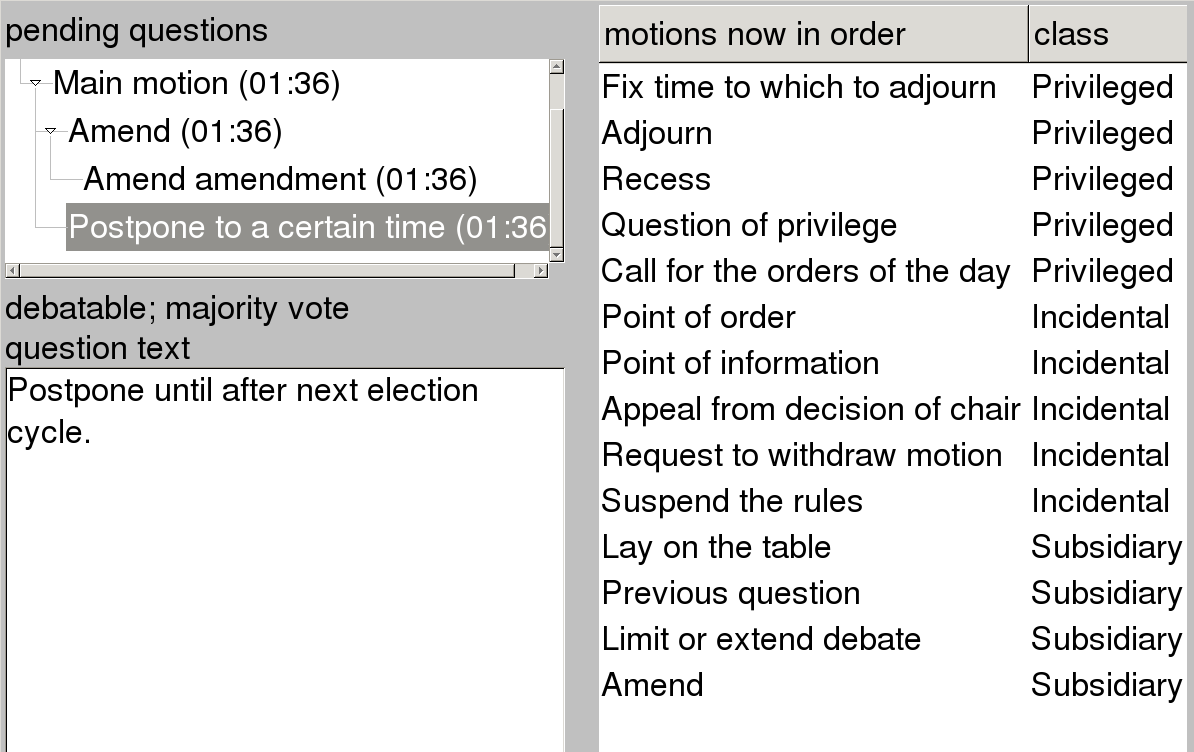
\includegraphics[scale=.42]{group}
\caption{The group interface. The tree of \emph{currently pending motions} is in the upper-left corner, with the \emph{rules} and \emph{text} of the immediately pending motion below. The list of \emph{motions currently in order} is on the right.}
\label{fig:group-interface}
\end{figure*}

\subsection{The Group Interface}

Figure~\ref{fig:group-interface} depicts the group interface, designed for a large shared display such as provided by a digital projector. The group interface provides a list of \emph{motions currently in order}, which depend on the meeting state---primarily on which motions are currently pending. A tree diagram displays the \emph{currently pending motions} and how they are related. The immediately pending motion is always at the bottom of the diagram, and the \emph{rules} relating to it and its \emph{text} are below.

\begin{figure*}[t]
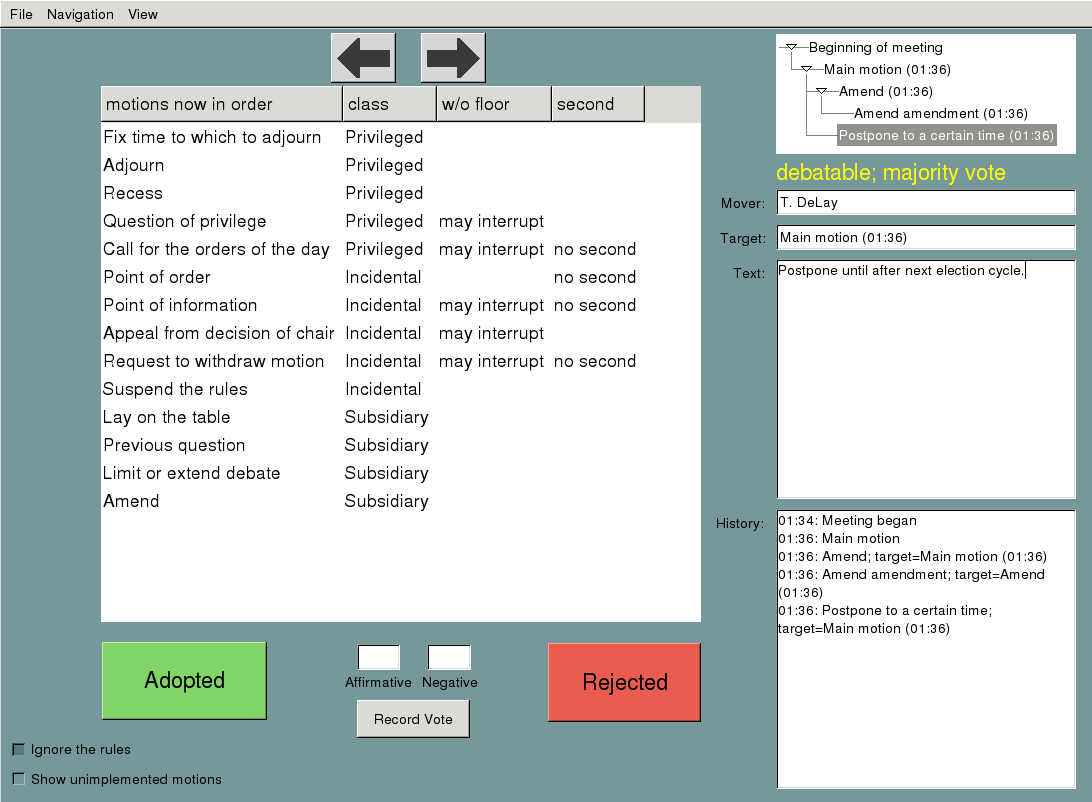
\includegraphics[scale=.46]{user}
\caption{The user interface. The list of \emph{motions currently in order} is on the left. The \emph{back} and \emph{forward} buttons are above. The \emph{adopted} and \emph{rejected} buttons and the \emph{vote-entry components} are below along with the \emph{ignore rules} checkbox. The tree of \emph{currently pending motions} is in the upper-right corner; below it are the \emph{rules} and the motion-detail fields: \emph{mover}, \emph{target}, and \emph{text}. The \emph{event log} is in the bottom-right corner.}
\label{fig:user-interface}
\end{figure*}

\subsection{The User Interface}

Figure~\ref{fig:user-interface} depicts the user interface, designed for a single user such as an organization's secretary. The user interface provides all the elements of the group interface, but allows interaction with them, and provides other interactive elements as well.

The user may activate any of the \emph{motions currently in order} to indicate a motion has been made in the meeting. The \emph{vote-entry components} comprise text fields for the number of affirmative and negative votes and a button that, when pressed, records the counts and the result based on the proportion required. \emph{Adopted} and \emph{rejected} buttons allow the user to indicate the fate of the immediately pending motion directly when votes are not counted. \emph{Back} and \emph{forward} buttons navigate through meeting history, providing a multiple undo/redo mechanism critical for usability.

The \emph{currently pending motions} in the tree diagram can be selected, populating several other fields with information about the selected motion. In addition to the \emph{text} of the motion, these also include its \emph{mover} and its \emph{target}. All these fields are editable by the user.

The interface also provides an \emph{event log} with a record of each motion in the order it was moved, and whether it was adopted or rejected.

As explained in Section~\ref{sec:live-setting}, the software must not break down under aberrations from the rules, but rather must continue to track meeting state. Hence the interface provides an \emph{ignore rules} checkbox that allows the user to record actions and motions despite these being out of order according to the module's interpretation of the rules.

\subsection{The Parliament Module}
 
\emph{Parliament} \cite{shanks:parliament} is an open-source software module that implements the logic and bookkeeping functions necessary for the function of parliamentary procedure, and is embedded in the application described here. This prototype is the first application of Parliament, and is useful as an interactive testbed for the module's features. It is hoped that Parliament will eventually be used in other settings, especially for online deliberation.
 
The Parliament module keeps track of meeting state. Meeting state includes data such as which motions are currently pending, the relationships between these motions, which motions are valid at the present time, and which motions have been adopted or rejected earlier in the meeting.

\subsubsection*{Parliament's Rule Specification}

The Parliament module does not incorporate the details of parliamentary procedure, such as the motions and customs described in Robert's Rules of Order. Instead, Parliament requires an external rule specification, allowing the user or developer to modify the rules independently and even to develop whole new rule systems. The independently modifiable rules simplifies the task of adapting the software for different parliamentary authorities or custom rules.

Much work has gone into creating the (partial) working specification of Robert's Rules of Order; certainly more than has gone into the interface design. The specification began from Henry Prakken's formalization \cite{prakken:formalizing}, which he kindly provided in machine-readable form. One aspect missing from Prakken's formalization is the notion of precedence; getting this right is both laborious and crucial to the goals outlined here.
 
\section{Preliminary Experience}  % .75

% preliminary experience
%   used at one meeting of GSAUCSD
%   lessons learned

The prototype system described in Section~\ref{sec:implementation} has been pilot-tested once in a live meeting of the Graduate Student Association of UCSD. Some important lessons were learned from this preliminary experience, including insights leading to the material in Section~\ref{sec:caveats}.

One problem encountered, for example, was with the physical arrangement of the room. Since the members spend much of the meeting looking in the direction of the chair, who faces them, it seemed fitting to place the projected display behind the chair. However, this meant the chair could not see the display. When the display accidentally diverged from the chair's statements, this made it more difficult than necessary to detect and fix.

A possible solution is for the operator of the interface to sit next to the chair. In this case, though the chair cannot see the projected display, he or she will be able to see the computer screen. 

Another lesson is that as soon as a computer and projector are introduced into a meeting, the group may well want to commandeer it for their own purposes. Members of GSAUCSD asked before the meeting if they could use the setup to display the text of bills they were to consider. During the meeting, a member requested display of a display a section of their constitution, which is published on the World-Wide Web. Although the system offers no support for the display of external documents, any system on which it runs will likely have other applications suitable for this task.

\section{Future Work}  % .75

The prototype implementation and preliminary experience reported here are intended to be only the beginning of this investigation. Future work will include more in-depth evaluation and iterative development sensitive to lessons from real use.

\subsection{Evaluation}

More experience using the system in live meetings will be critical to ongoing development of the software and the ideas it embodies. Evaluation of the system faces many challenges common to other groupware \cite{grudin:groupware}. Importantly, however, the system can be introduced to existing assemblies in their natural environments with a minimum of explanation so long as experimenters run the system. Evaluation with organizations' secretaries running the system is a next step.

Objectives to be judged by further evaluation include whether the system improves conformance to the rules, whether it increases participation, and whether it leads to greater satisfaction with the outcomes and with meetings as a whole. Through careful expert ethnography, it may be possible to quantify rule conformance, yielding an objective measure of success. Patterns of participation, both in debate and in motion-making, likewise can statistically analyzed. Qualitative evaluation might include asking participants whether they experience increased awareness of the procedures, and whether they feel more confident about engaging the process when the system is in use.

\subsection{Development}

Features proposed for the software include, roughly in order of priority:

\begin{itemize}
 \item a flexible report tool that can automatically produce a draft of official minutes;
 \item indicating business on the table and taking business from the table;
 \item support for orders of business and agendas; and
 \item floor control, speakers lists, and limits on debate.
\end{itemize}

Another target within grasp, in order to test the system's flexibility, is to develop other rule specifications based, for example, on \textit{the Standard Code of Parliamentary Procedure} \cite{sturgis:standard} or special rules added to Robert's Rules of Order in an organization's bylaws.

\subsection{Distant Possibilities}

Conceivable but further off are support for direct electronic input from participants and interoperation with online deliberation systems.

Electronic meeting systems described in the literature often have computer terminals for all participants \cite{nunamaker:electronic}. A parliamentary-procedure system of this sort could provide the information available on the public display, but also enable access to more details on the motions and rules relating to them. Participants could give input such as votes and written motions electronically. The system could even automatically mediate requests for the floor \cite{stodolsky:automatic}.

The ability for software supporting face-to-face deliberation to interoperate with online deliberation systems of the future is a worthy goal. Data-format compatibility is a good target. Unfinished business from face-to-face meetings could be exported to online deliberation and resumed at the next meeting; business could be seamlessly ``referred to online committee'', carrying with it all attached motions and other relevant information. This kind of confluence is encouraged by modular support like Parliament \cite{shanks:parliament} that can be embedded in a variety of applications.

\section{Relation to Other Work}  % .5

There is a considerable body of work on electronic meeting systems and systems to support group decision making, whether face-to-face or otherwise, but little work has focused on parliamentary procedure.

\subsection{Group Decision Support Systems}

% idea specifically proposed by DeSanctis & Gallupe [ref]
%   classified in Level 3 (describe)

A \emph{group decision support system (GDSS)} employs technology to facilitate, and hopefully to improve, group decision making. A GDSS is \emph{groupware}, in that it is designed for multiple people working collaboratively. As a field, GDSSs are related to \emph{decision support systems (DSS)}, although the latter typically focus on the information gathering and analysis tasks an individual decision maker might engage in.

A GDSS to apply parliamentary procedure was envisioned at least as early as 1987 by DeSanctis and Gallupe \cite{desanctis:foundation}. In the nomenclature of their foundational paper, such a system is called a \emph{Level 3 GDSS}, the highest level involving the most dramatic intervention in the group's decision process. While Level 1 GDSSs aim only to facilitate communication and Level 2 GDSSs passively offer tools and models, Level 3 GDSSs actually apply rules regulating the decision process.

%   system described here also uses elements of L1, but not L2

Many actual and proposed features of the parliamentary-procedure software described in this paper belong to DeSanctis and Gallupe's Level 1: a large common viewing screen, public display of votes, continuous display of agendas, automatic timely reminders about agenda items, computer terminals for group members, anonymous electronic voting.

The possibility of a system to support face-to-face parliamentary procedure had been suggested, and many useful components conceived, but no such system appears to have emerged. In fact, DeSanctis and Gallupe advocated delaying work on Level 3 systems until lower-level systems were better understood. One reason for this was their belief that the ``technology required to build a Level 3 GDSS shell is not yet available,'' possibly because they expected it to be ``expert-system based'' and to ``provide advice on selecting or defining rules.''

Kraemer and King, in their survey of systems for cooperative work and group decision support \cite{kraemer:computer-based}, argue that ``most of the efforts to apply these technologies have affected decision processes too much or too little to provide a good assessment of their effects.'' On one hand, audiovisual presentation and teleconferencing technologies ``affect decision meetings only by speeding up certain common tasks [\ldots] or adding flexibility [\ldots] Neither claims to improve the quality of decision making appreciably.'' On the other hand, approaches that prescribe structured protocols and collaboration techniques ``attempt to improve the actual process and consequence of decision meetings, but they nevertheless impose the designers' views of the decision process on the participants.''

% Kraemer and King GDSS taxonomy: decision conference

The support for parliamentary procedure proposed herein aims to improve group decision making without externally imposing structure. Many organizations have already adopted a parliamentary authority such as Robert's Rules of Order, usually in their bylaws or such governing documents. Our approach is to support group understanding and use of rules that already apply; it is an effort to improve the practice, rather than the theory, of group decision making.

% D&G ``Robert's rules of order, or discussion procedures self-designed by the group''
% D&G ``Legislative Session ... meeting proceedings can be recorded''
% D&G ``Computer-Mediated Conference ... large, dispersed groups responsible for decisions''
% D&G ``users must have extended experience with GDSS before the effectiveness or ineffectiveness of systems design can be fully assessed.''
% D&G ``Performance/Satisfaction Tradeoff ... high quality decisions, or a high sense of satisfaction ... improve the efficiency and effectiveness of group decision making

% original motivation for Parliament: online deliberation
%   "Doug Schuler proposed in his 1996 book New Community Networks that
%    Roberts Rules of Order could be used as a basis for online deliberation."

% face-to-face meetings have useful properties
%   simultaneous shared attention, intersubjectivity
%     rich communication channel, quick exchange, synchronizing
%   live meetings complement online collaboration
% integrate in-person with online deliberation

% \subsection{EMS papers}
% 
% Nunamaker \textit{et al.} \cite{nunamaker:electronic}
% 
% Hayne \cite{hayne:facilitators}

\subsection{Work Related to Robert's Rules of Order}

Some aspects of parliamentary procedure are oriented toward a live, in-person environment; but the underlying principles and many of the rules can be applied to decision-making groups using various other modes of communication.

One group designed a document-based collaboration system based on an ``agenda item life cycle'' inspired by Robert's Rules of Order \cite{chang:rule-mitigated}.. Based on this model, they built a client-server architecture for spatially distributed collaboration, both synchronous and asynchronous \cite{chang:rule-mitigated,zhang:rule-mitigated}.

Other researchers have investigated adapting Robert's Rules of Order for use in the context of computer-mediated communication. Horan and Benington describe a protocol for conducting electronic deliberations by e-mail in academic committees that use Robert's Rules of Order \cite{horan:protocol}. They assume that users will implement the protocol, but software could automate some of what they recommend.

\emph{Robert's Rules in Motion}\footnote{\url{http://imovethat.com/}} is a commercially available single-user application that simulates meetings in order to train the user in the use of parliamentary procedure. It contains much of the logic needed for other parliamentary-procedure applications, but no code nor programmable module is available.

% Chang \textit{et al.} \cite{chang:rule-mitigated}
% 
% not really the rules of parliamentary procedure
%   but a simple "agenda item life cycle" inspired by RRO proceedings
% extended RRO for electronic collaboration
%   eliminate unique floor, allow concurrency
%     discussion threads
%   limit on nesting of amendments is unnecessary
%   abolition of motion to recess
%   electronic meeting may be adjourned only once, when the work is concluded
%   provide a mechanism for modifying the agenda
%   motions to modify assembly membership

% \subsection{OD papers}

% Davies \textit{et al.} \cite{davies:community}

% Witschge \cite{witschge:online}

% Davies \textit{et al.} have built an online deliberation environment, \emph{Deme} \cite{davies:online}, primarily to supplement the activities of groups that already meet face-to-face.

% \subsection{OD projects}

% Robert's Rules Assembly\footnote{\url{http://grace.evergreen.edu/~powmat25/RR/Home.html}}

% e-Liberate\footnote{\url{http://trout.cpsr.org/program/sphere/e-liberate/about.php}}

% Public Sphere Project\footnote{\url{http://trout.cpsr.org/program/sphere/}}

% Deme\footnote{\url{http://groupspace.org/}}

% \subsection{Other projects}

% GroupSystems\footnote{\url{http://www.groupsystems.com/}}

% ActionForum.com\footnote{\url{http://www.actionforum.com/}}

% Facilitate.com\footnote{\url{http://facilitate.com/}}

\section{Conclusions}  % .25

The technology described herein shows promise for improving the practice of parliamentary procedure in face-to-face meetings. Assemblies with members not well practiced in the rules can especially benefit from the support of such a system.


Software support for parliamentary procedure fills a unique niche among similar research. By supporting group work while having a single user operating the interface, it eludes many pitfalls of many groupware applications and suggests possibilities for meeting the challenges they face. By aiming to improve group decision making without externally imposing structure, face-to-face parliamentary-procedure software offers opportunities to study effects on groups that were obscured by the more dramatic interventions of other group decision support systems.

Parliamentary-procedure software should run on common portable computers, and be easy for any organization's secretary to learn and use, streamlined enough to keep pace with live meetings, and flexible enough to handle the adaptive circumvention of rules that inevitably occurs in real assemblies. In addition, the software should generate a record from which official minutes can be produced, and which may in the future be a medium for interoperation with online deliberation systems.

Preliminary experience with a prototype system in real meetings has met with enthusiastic response and has yielded valuable insights into the design and use of future systems. Further development and experimentation following this initial excursion is warranted and underway.

\section{Acknowledgments}  % .25

The Center for Research in Computing and the Arts\footnote{\url{http://crca.ucsd.edu/}} generously lent the use of their digital projector for the preliminary experience reported here.

\bibliographystyle{abbrv}  % 1.0
\bibliography{../parliprosoft,../uid}
 
\end{document}
